\chapter{Critique of the Physical Concepts of the Particle Picture}
\chapterprecis{Werner Heisenberg}

\makeoddhead{myheadings}{\emph{Heisenberg}}{}{\thepage}
\makeevenhead{myheadings}{\thepage}{}{\emph{Critique of the Physical Concepts of the Particle Picture}}

\renewcommand{\theequation}{\arabic{equation}}



\section*{The Physical Principles of the Quantum Theory\footnote{{[}\emph{Die
  Physikalischen Prinzipen der Quantentheorie}, Leipzig (1930); also
  \emph{The Physical Principles of the Quantum Theory}, trans. C. Eckart
  and F. C. Hoyt, Chicago (1930). The present selections were translated
  1995 by C. Burke and E. Brann, slightly revised in 2007 by H. Higuera
  and in 2014 by R. Druecker.{]}}\\
  {\large Werner Heisenberg}}

\subsection*{CHAPTER II\\
CRITIQUE OF THE PHYSICAL CONCEPTS OF THE PARTICLE PICTURE}

\subsubsection*{§I. The Indeterminacy Relations}

The concepts of position, velocity, and energy have been derived from
simple experiments of everyday experience, in which the mechanical
behavior of macroscopic bodies is described by these words. These
concepts were then carried over to electrons, since in some fundamental
experiments electrons show a mechanical behavior similar to objects of
everyday experience. But since we know that this similarity exists only
in a limited region, the range of applicability of the concepts of the
particle picture must be restricted in a corresponding way. According to
Bohr,\footnote{N. Bohr, \emph{Nature}, \textbf{121}, 580, 1928. {[}Note taken
  from English edition, giving citation to English version of Bohr's
  article.{]}} one arrives at this restriction in the simplest way by
recalling that all intuitable facts (i.e., facts describable in space
and time) of atomic physics must \emph{also} be describable in a wave
picture.

The following considerations apply equally to each of the three space
co-ordinates of the electron and are therefore carried out for only one.
The fact that the position of an electron is known with a certain
exactness $\Delta$\emph{x} {[}at the time \emph{t}{]} can obviously be
described in the wave picture by a wave function whose amplitude is
significantly different from zero only in a small range of approximate
magnitude $\Delta$\emph{x}. A wave function constructed in this way can always
be thought of as composed of a number of partial waves which interfere
with each other in such a way as to reinforce one another within the
small spatial range \emph{$\Delta$x} but cancel one another everywhere outside
that range. Such a configuration is called a \emph{wave packet}. A
general mathematical proposition states that it is always possible,
through appropriate composition of the individual partial waves, to
build up a wave packet of any desired shape. In the course of time such
a wave packet will in general change its size and shape and, apart from
special cases, will ultimately be dispersed over the whole of space. The
velocity of the electron likewise corresponds to the velocity of the
wave packet; however, no exact velocity can be defined for the wave
packet because, as was said, besides its forward motion, it also spreads
and disperses itself. This dispersion thus occasions an indeterminacy in
the definition of the momentum (mass times velocity) of the amount, say,
$\Delta$\emph{p}. Now, from the simplest laws of optics, together with the
equations
\begin{equation*}
{[}\lambda = \frac{h}{p} \quad\quad \text{and} \quad\quad v_g = \frac{h}{\mu\lambda_0}{]}
\footnote{{[}Heisenberg derives these equations in an
  appendix and references them here rather than writing them out. For
  further details see footnote 6 below.{]}}
\end{equation*}
it can be derived that
\begin{equation}
\Delta x\Delta p_x \geq h. % eqn (1)
\end{equation}

For, think of the wave packet as being composed out of the superposition
of plane {[}sinusoidal{]} waves, whose wave-lengths are to lie in the
neighborhood of $\lambda_0$. Then, on the whole,
$n = \Delta x/\lambda_0$ crests or troughs fall in the region
inside the packet. Outside the packet the plane waves are to cancel each
other by interference; this is possible if, and only if, the totality of
component plane waves contains some for which at least $n + 1$
waves fall in the critical range. This gives
\begin{equation*}
\frac{\Delta x}{\lambda_0 - \Delta\lambda} \geq n + 1 ,
\footnote{{[}The waves of
  longer and shorter wavelength must reinforce each other at the center
  of the packet and interfere at each end. Hence they must be out of
  coincidence by one-half wavelength at each end, which is only possible
  if the shorter waves are contained at least one more time than are the
  longer waves in the same distance $\Delta$\emph{x}. If there are
  $n=\Delta x/\lambda_0$ of the longer waves of length $\lambda_0$ in the
  packet, then there must be at least $n + 1$ of the shorter waves
  of length $\lambda_0 - \Delta\lambda$ within the same region $\Delta x$.{]}}
\end{equation*}
where $\Delta\lambda$ indicates approximately the range of wave-lengths which
is necessary for the representation of the packet. Consequently
\begin{equation}  % eqn (2)
\frac{\Delta x\Delta\lambda}{\lambda^2_0} \geq 1 .\footnote{{[}From the 
  inequality at the end of the previous note,
  \begin{equation*}
  \frac{\Delta x}{\lambda_0-\Delta\lambda} \geq n + 1 = \frac{\Delta x}{\lambda_0} + 1,
  \end{equation*}
  collecting algebraic terms to the left and adding gives,
  \begin{equation*}
  \frac{\Delta x\Delta\lambda}{\lambda_0(\lambda_0-\Delta\lambda)} \geq 1 ,
  \end{equation*}
  which can be approximated to inequality (2) if $\Delta\lambda$ is
  sufficiently small compared to $\lambda_0$.{]}}
\end{equation}
On the other hand, the group velocity of the waves is
\begin{equation}
v_g = \frac{h}{\mu\lambda_0} .  % eqn (3)
\footnote{{[}As just mentioned, Heisenberg derives equation (3) in an
  appendix. Here $\mu$ is the mass of an electron. Now if in de
  Broglie's $\lambda = h/p (=h/\mu v)$ one stipulates that the de
  Broglie wavelength of the \emph{electron} is ``the''
  $\lambda_0$ of the \emph{packet} and that the velocity
  of the electron equals the group velocity, one gets $\lambda_0=h/\mu v_g$, from
  which eq. (3) follows immediately. But Heisenberg actually derives eq.
  (3) \emph{directly from the Schrödinger wave equation} and,
  without relying on ``particle'' concepts. As he writes, ``The wave
  theory does not consider electrons, {[}but{]} merely universal
  constants of the wave equation.''{]}}
\end{equation}
The dispersion of the packet corresponding to the range $\Delta\lambda$ is
therefore characterized by {[}a range of velocities{]}
\begin{equation*}
\Delta v_g \approx \frac{h}{\mu\lambda_0^2}\Delta\lambda .
\footnote{{[}If one does \emph{not} impose assumptions from the
  particle picture, then in the packet \emph{both} the longer \emph{and}
  the shorter waves have an equal claim to be considered ``the''
  wavelength for purposes of equation (3). That equation is already
  written for the longer wavelength $\lambda_0$. Were it instead to be
  written for the shorter wavelength, $\lambda_0 - \Delta\lambda$, there would
  be determined a different group velocity,
  \begin{equation*}
  v'_g = \frac{h}{\mu(\lambda_0-\Delta\lambda)}
  \end{equation*}
  and the difference between $v'_g$ and $v_g$ is the ``range of
  velocities'' $\Delta v_g$. Thus
  \begin{equation*}
  \Delta v_g =\frac{h}{\mu(\lambda_0-\Delta\lambda)}-\frac{h}{\mu\lambda_0} =
  \frac{h\Delta\lambda}{\mu\lambda_0(\lambda_0-\Delta\lambda)}\approx\frac{h\Delta\lambda}{\mu\lambda^2_0}
  .{]}
  \end{equation*}
}
\end{equation*}
  By definition $\Delta p_x = \mu\Delta v_g$, and therefore by
  equation (2),
\begin{equation*}
  \Delta x\Delta p_x \geq h
  . \footnote{{[}Substituting from the
  equation for $\Delta v_g$, $\mu\Delta v_g = \mu\frac{h}{\mu\lambda_0^2}\Delta\lambda
  = h\frac{\Delta\lambda}{\lambda^2_0}$. Therefore, $\Delta x\Delta p_x = h\frac{\Delta x\Delta\lambda}{\lambda^2_0}$; 
  that is, by equation (2), $\Delta x\Delta p_x$ equals $h$ times something $\geq 1$.{]}}
\end{equation*}\\
\centerline{* * *}
%
The indeterminacy relations [\ldots] specify the limits within which the
concepts of the particle theory can be applied. Any use of the words
``position'' or ``velocity'' with an exactness exceeding that indicated
by equation (1) is just as empty of content as the use of words whose
sense has not been defined.\footnote{In this connection one should
  particularly remember that the human language quite generally permits
  the construction of sentences from which no consequences follow and
  which are therefore completely empty of content, although these
  sentences produce a kind of intuitable representation. For example,
  the assertion that besides our world there exists another world, with
  which any connection is impossible \emph{in principle}, does not lead
  to any inference; nevertheless, accompanying this statement a kind of
  picture arises in the imagination. Obviously such a statement can
  neither be proved nor disproved---one should be especially careful in
  the use of the expression ``in actuality'' since it very often leads
  to assertions of the type just discussed.}\\
\centerline{* * *}
%
\subsubsection*{§2. Confirmation of the Intedeterminacy Relations using Various
Measuring Devices}

The indeterminacy relations relate to the degree of exactness in our
present (simultaneous) knowledge of the various quantum-theoretical
magnitudes. Since these relations do not restrict the exactness, for
example, of a position measurement alone or a velocity measurement
alone, their effect expresses itself only in the fact that each
experiment that makes possible a measurement of, say, position,
necessarily disturbs the knowledge of the velocity to a certain degree.
Let us suppose, for example, that the velocity of a {[}free{]} electron
is exactly known, while the position is completely unknown. Then every
subsequent observation of the position must alter the momentum of the
electron, and this alteration must be indeterminate by an amount such
that after the experiment is carried out our knowledge of the electron's
motion is limited by the indeterminacy relations. This will be confirmed
in what follows, using some experiments as examples. But first let it be
remarked that the indeterminacy relations evidently do not refer to the
past. For if the velocity of the electron is known to begin with, and
subsequently the position is exactly measured, then the electron's
positions for the time \emph{before} the measurement of position may
also be exactly calculated. For this previous time, the quantity
$\Delta p\Delta x$ will be smaller than the usual limiting value. This
knowledge of the past, however, is of a purely speculative character,
since---because of the change in momentum caused by the position
measurement---it can in no way enter as an initial condition in any
calculation concerning the future of the electron, and never makes an
appearance in any physical experiment at all. It is thus a pure matter
of taste whether or not one is to ascribe to such a calculation
concerning the past of the electron any physical reality.

\begin{figure}[h] % Figure 5
  \begin{center}
    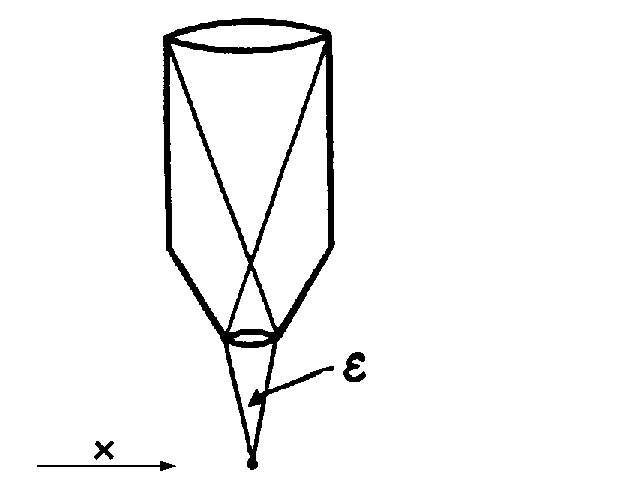
\includegraphics[width=1.875in,height=1.40625in]{images/10_heisenberg/image015.png}
  \end{center}
  \caption*{\emph{Figure 5.}\footnote{{[}The figure is that of the 1930 Chicago edition and
  corrects an error in the Leipzig edition.{]}}}
\end{figure}
%\includegraphics[width=1.875in,height=1.40625in]{media/image18.png}

a) \emph{Determination of the position of a free particle.}---As a first
example of the disturbance of the knowledge of a particle's momentum by an
apparatus for measuring position, we choose the position measurement by
means of a microscope.\footnote{N. Bohr, \emph{loc. cit.}} Let the
electron be moving at such a distance under the objective of the
microscope that the cone of rays scattered from it has an angular
opening $\varepsilon$. Let the wave-length and frequency of the light
illuminating the electron be $\lambda$ and $\nu$; then the exactness
in the position measurement of the $x$-direction (see Fig.\ 5)
according to the {[}limit on resolving power of any optical
instrument{]} is:\footnote{{[}The resolving power of a lens is limited
  by the aperture of the lens, since any small opening will diffract any
  light it transmits. If the central maxima of the diffraction patterns
  of two objects then overlap to any great extent, those objects will be
  indistinguishable through the lens. The separation, $\Delta x$, at
  which two ``point'' objects can no longer be distinguished sets a
  limit to our ability to determine the position of an object with a
  microscope---a limit which depends on the angular aperture of the
  objective lens and the wavelength of the illuminating light. A
  derivation of equation (16) is given in the Note at the end of this chapter.{]}}
%
\begin{equation*}\tag{16}
\Delta x \approx \frac{\lambda}{\sin \varepsilon} .
\end{equation*}
%
But for a position measurement to be possible, at least one photon must
be scattered from the electron and pass through the microscope to reach
the eye of the observer. From this one photon, the electron receives a
Compton recoil\footnote{{[}Recall that the interaction of light
  with electrons can be understood as an \emph{elastic collision}
  between electrons and photons if the photons of energy
  $e= h\nu$ are also assigned momentum of amount $p = h/\lambda$.

  In the sketch, a photon after rebounding from a particle will have
  momentum $h/\lambda$. If it enters the microscope it must fall
  within the angle $\varepsilon$ and therefore will carry away momentum
  $px$ in the $x$-direction, which can be as little as
  \emph{zero} or as much as $(h/\lambda)\sin \varepsilon$. But since the
  direction of any particular photon cannot be distinguished by the
  microscope, the momentum of the particle is unknown within a range
  equal to $(h/\lambda)\sin \varepsilon$.{]}
  \begin{center}
    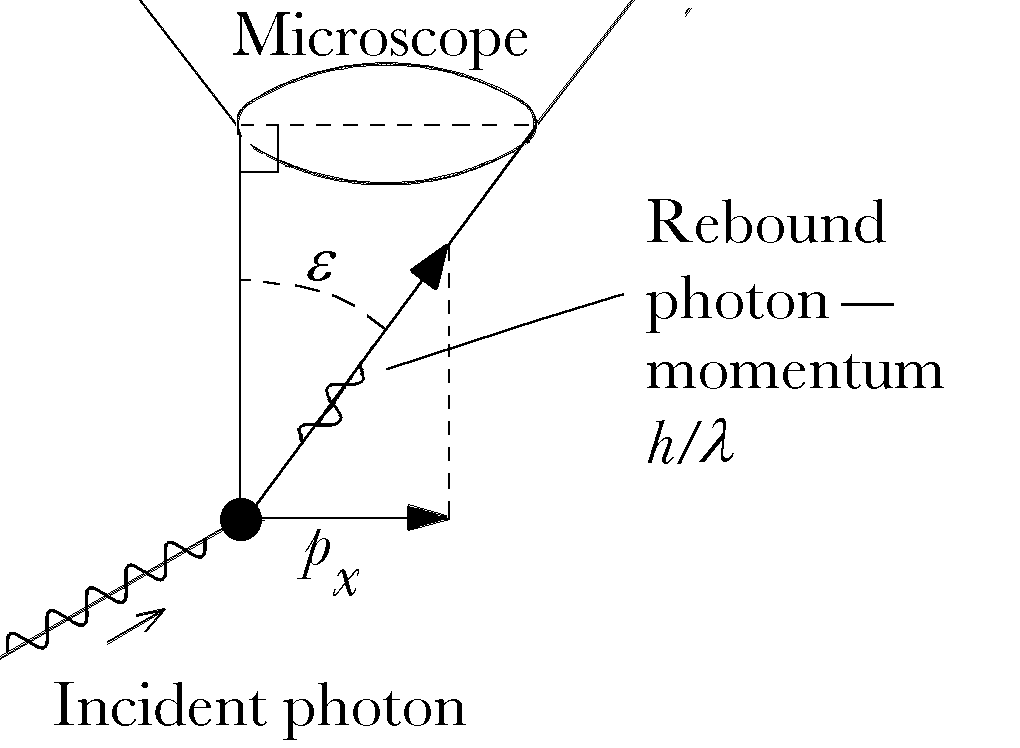
\includegraphics[width=1.7in,height=1.24667in]{images/10_heisenberg/image054.png}
  \end{center}
  } of order of magnitude
$h/\lambda$. The recoil cannot be known exactly, since within the bundle
of rays (of angular opening $\varepsilon$) the direction of the photon
{[}entering the microscope{]} is unknown.\footnote{{[}There is a lens
  across the aperture. If the microscope is focused properly, then
  according to ray-optics \emph{wherever} the ``ray'' of light passes
  through the lens, it will be refracted onto the same point on the
  detecting screen.{]}} Thus there will be an uncertainty of the recoil
in the $x$-direction of amount
%
\begin{equation*}\tag{17}
\Delta p_x \sim \frac{h}{\lambda}\sin \varepsilon % eqn (17)
\end{equation*}
%
and it follows for the knowledge of the electron's motion after the
experiment that
%
\begin{equation*}\tag{18}
\Delta x\Delta p_x \sim h. % eqn (18)
\end{equation*}
%

Objections may at first be raised against this derivation: The reason
for the indeterminacy of the recoil is, after all, that it is unknown
which path within the bundle of rays the photon takes. One might thus
try to determine this path by making the whole microscope movable and
measuring the recoil that it receives from the photon. But this will not
help to circumvent the indeterminacy relations; for there then
immediately arises the question of the position of the microscope, and
the position and momentum of the whole microscope will also be subject
to equation (18). To be sure, the measurement of the position of the
microscope could be neglected altogether if the electron and a fixed
scale could be simultaneously observed through the movable microscope.
But then one observation would require the simultaneous passage of at
least two photons through the microscope to the observer---one from the
scale and one from the electron---and a measurement of the recoil of the
microscope would no longer yield information about the photon coming
from the electron, and so on.

The whole discussion of this experiment characteristically makes use of
the wave picture and the particle picture simultaneously. Here we make
use of that duality essentially in the theory of radiation; for on the
one hand we speak of bundles of rays and the laws of optics, and on the
other hand, of photons and the recoils caused by them.

%
\begin{figure}[h] % Figure 6
  \begin{center}
    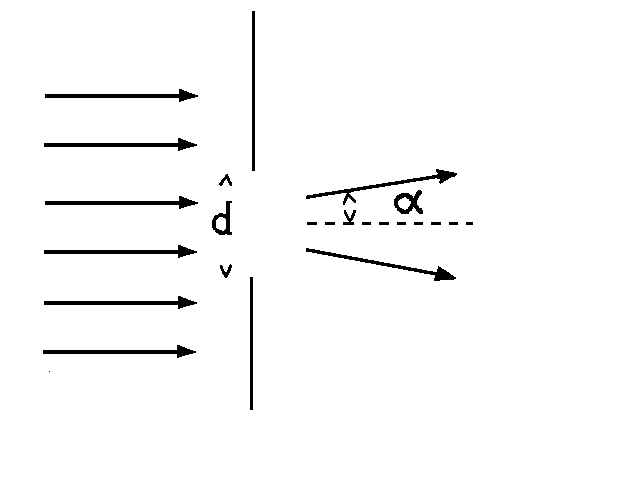
\includegraphics[width=1.875in,height=1.4414in]{images/10_heisenberg/image021.png}
  \end{center}
  \caption*{\emph{Figure 6.}\footnotemark}
\end{figure}
\footnotetext{[The figure is that of the 1930 Chicago edition and
  corrects an error in the Leipzig edition.]}
%

Another simple determination of position can be performed in the
following way: Again let the velocity of the electron be completely
known. Consider a set of possible paths which an electron might take in
approaching a screen that contains a slit of
width $d$ (Fig. 6). If the electron passes through this slit, then evidently
its position in the direction parallel to the screen is fixed with
exactness $\Delta x = d$. If the oncoming electron is represented
by a plane de Broglie wave, however, one sees immediately that
diffraction will occur. The emerging wave will have a finite angular
opening $\alpha$ which, by the simplest laws of optics,\footnote{{[}``The
  simplest laws of optics:'' Heisenberg refers to the expression for
  single-slit diffraction, $\sin \theta_1 = \lambda/d$,
  where $\theta_1$ is the half-width of the central maximum (see the Note
  at the end of this chapter).{]}} will be given by
%
\begin{equation*}\tag{19}
\sin \alpha \sim \frac{\lambda}{d} , % eqn (19)
\end{equation*}
%
where \emph{$\lambda$} is the wave-length of the de Broglie waves. Thus the
momentum of the electron parallel to the screen, after the electron's
passing through the slit, is uncertain by an amount
%
\begin{equation*}\tag{20}
\Delta p_x = \frac{h}{\lambda}\sin \alpha % eqn (20)
\end{equation*}
%
since $h/\lambda$ is the momentum of the electron in the direction of the
beam. Then, since $\Delta x = d$, it follows that
%
\begin{equation*}
\Delta x \Delta p_x \sim h.
\end{equation*}
%
In this derivation, although no use is made of the wave-particle duality
in the theory of radiation, it is indeed used in the theory of matter.\\
\centerline{* * *}
%
\subsection*{CHAPTER IV\\ 
THE STATISTICAL INTERPRETATION OF QUANTUM THEORY\footnote{{[}\emph{Nature}, 121,
  580, 1928. Again, citing the English version.{]}}}
\centerline{* * *}

\subsubsection*{§3. Bohr's Concept of Complementarity}


The world of concepts derived from everyday experience was for the first
time left behind in Einstein's relativity theory. It became apparent
that the ordinary concepts could only be applied to processes in which
the velocity of the propagation of light could be regarded as
practically infinite. The experiential material which has been refined
through modern experimental physics thus necessitated the revision of
received concepts and the development of new ones; but our thinking
could adjust itself only slowly to that extended range of experience and
the world of its concepts; and therefore relativity theory itself
seemed at first abstract and alien. As is clear from what has been said,
the experiences from the world of atoms compel us to an even more
extensive renunciation of hitherto customary concepts. Indeed, our
ordinary description of nature and especially the thought of a strict
lawfulness in the processes of nature rest on the assumption that it is
possible to observe phenomena without appreciably influencing them. To
co-ordinate a determinate cause to a determinate effect has a meaning
only when we can observe effect and cause without simultaneously
disturbing the process by our intervention. The law of causality in its
classical form can thus, by its nature, be defined only for isolated
systems. But in atomic physics there is in general connected with each
observation a finite disturbance that is to a certain degree
uncontrollable, as was from the very beginning only to be expected in
the physics of what are in principle the smallest units. Since, on the
other hand, every space-time description of a physical process is
conditioned by the observation of the process, it follows that the
space-time description of processes on the one hand, and the classical
law of causality on the other, represent complementary and mutually
exclusive features of the physical event. What corresponds to this
situation in the formalism of the theory is the fact that while a
mathematical model of quantum theory exists, this model cannot be
interpreted as a simple connection of things in space and time. Through
this complementarity of the space-time description on the one hand, and
of the causal connection on the other, there arises moreover a peculiar
ambiguity in the concept ``observation'' in that it is left arbitrary
which objects are to be counted as belonging to the observed system and
which are to be regarded as means of observation. In the formalism of
the theory this arbitrariness has the consequence that often quite
heterogeneous methods can be used for the interpretation of a physical
experiment [\ldots]. But even if one accepts the arbitrariness mentioned,
the concept ``observation'' belongs strictly speaking to the world of
ideas drawn from our everyday experience. It can be carried over to
atomic phenomena only when due regard is paid to the limitation placed
on all space-time pictures by the indeterminacy relations. For every
observation is by definition bound to space and time; therefore, this
concept has meaning only within the boundaries specified by those
relations. It has already been mentioned that there are special cases in
which the requirements of the classical law of causality can be brought
into agreement with a spatio-temporal description to a certain
approximation. In general, however, the situation can be characterized
by something like the following diagram:

\begin{figure}[h] % Figure 5
  \begin{center}
    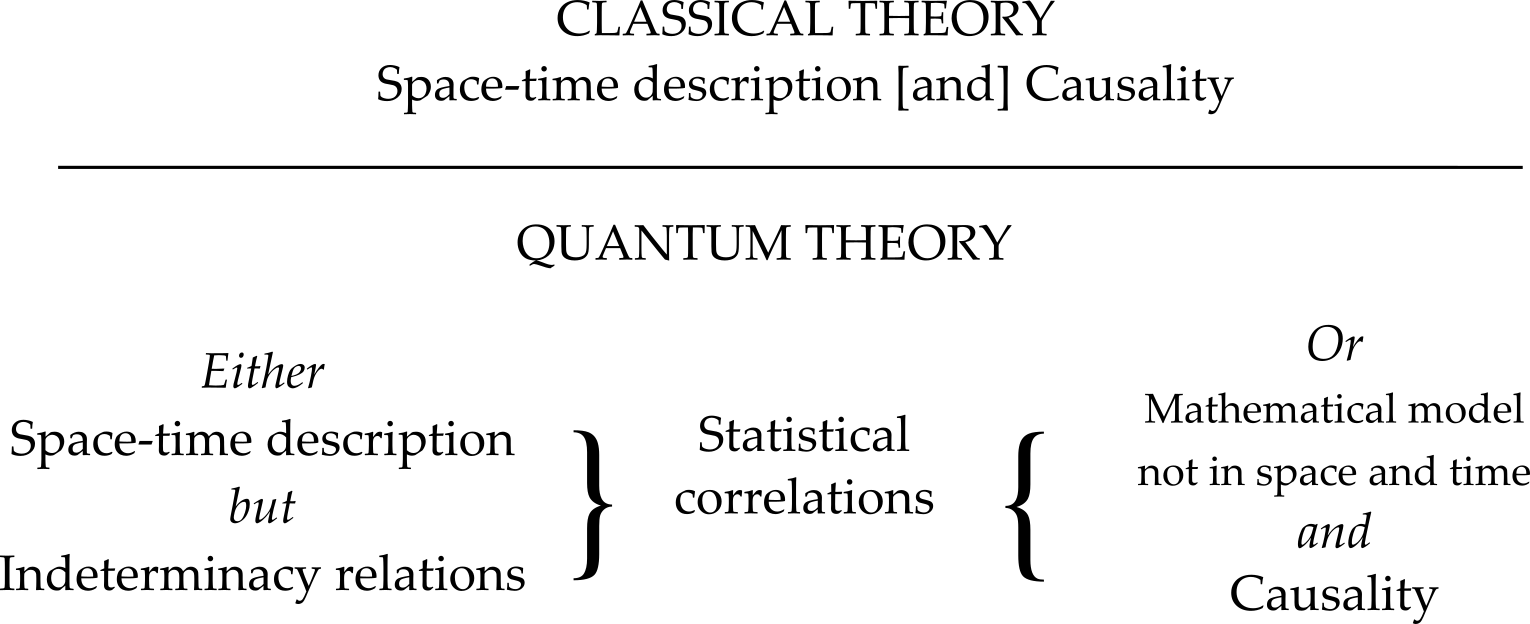
\includegraphics[width=5.1in,height=2.08in]{images/10_heisenberg/heisenberg-table.png}
  \end{center}
\end{figure}

It is only after attempting to adjust the formation of one's concepts
to this fundamental complementarity of space-time description and
causality, that one is in a position to judge whether the methods of
quantum theory are free of inconsistency [\ldots]. The adaptation of our
thought and our language to the experiences of atomic physics is indeed
associated with great difficulties, just as it had been for relativity
theory. In relativity theory the earlier philosophical discussions of
the problems of space and time proved to be very serviceable to this
adaptation. In a similar way one can profit in atomic theory from the
discussions, fundamental to all epistemology, concerning the
difficulties connected with the separation of the world into subject and
object. Quite a few abstractions which are characteristic of modern
theoretical physics will be found to have been already discussed in the
philosophy of past centuries. While these abstractions could in the past
be rejected as thought-play by the natural scientist intent only on
realities, the more refined experimental art of modern physics now
forces us to discuss them thoroughly.\\
\centerline{* * *}
%

\section*{M. BORN: THE PROBABILITY INTERPRETATION}

Physicists generally came to accept the mathematical formalism of the
$\Psi$ waves as initiated by de Broglie and developed by Schrödinger.
However, there was a lively debate over the \emph{interpretation} of
them. Einstein, for example, as we shall see later on, thought that, in
some sense, the $\Psi$ function did not give the complete account of
entities like electrons because it was based upon inadequate concepts of
classical physics.

Aside from this suggestion there seem to be, roughly speaking, three
possibilities. As was seen in Chapter \ref{ChDeB}, de Broglie thought of an
electron as simultaneously \emph{both} a particle \emph{and} a wave.
Secondly, one might hold that an electron is \emph{only} a wave, and not
a particle at all. De Broglie's second presentation of his idea of wave
mechanics suggests the following reasoning: Huygens and Young saw that
if wave optics is correct, there really are no light particles but only
light waves that appear as straight-line particle paths due to the
smallness of the wavelength in comparison with the size of the objects
with which the waves interact. So too it should be the case that if wave
mechanics is correct, there really are no material particles but only
$\Psi$ waves that appear as particles in certain situations. This is
the approach taken by Schrödinger. He considered that a particle was
simply a wave packet, and he associated the function $\Psi$ in a
certain way with the density of charge in space.

The third approach, the so-called ``Copenhagen interpretation,''
according to which an electron is \emph{either} a particle \emph{or} a
wave---in the sense that it exhibits now particle-like behavior, now
wave-like behavior---but never both simultaneously, was the one
developed by Bohr and Heisenberg.

The Copenhagen complementarity interpretation of the electron was joined
with an interpretation of the wave function $\Psi$ proposed by Max
Born. According to this interpretation, the wave function at any point
in space, $\Psi(x,y,z,t)$, is to be viewed as determining a
\emph{probability density}---that is, the probability, per unit volume,
of \emph{observing}\footnote{``Observing'' includes, for example, having
  a particle cause a glow on a screen at a point.} \emph{a particle}
very near that point.

In the following passage from his textbook,\footnote{\emph{Atomic
  Physics} (New York: Hafner, 1962), 96-100.} Born begins the
presentation of his interpretation by opposing that of Schrödinger:

\begin{quotation}
In the preceding sections we have had a series of facts brought before
us which seem to indicate unequivocally that not only light, but also
electrons and matter, behave in some cases like a wave process, in other
cases like pure corpuscles. How are these contradictory aspects to be
reconciled?

To begin with, Schrödinger attempted to interpret corpuscles, and
particularly electrons, as \emph{wave packets.} Al­though his formulae
are entirely correct, his interpretation cannot be main­tained, since on
the one hand, as we have already explained above, the wave packets must
in course of time become dissipated {[}see below{]}, and on the other
hand the description of the interaction of two electrons as a collision
of two wave packets in ordinary three‑dimensional space lands us in
grave difficulties.\footnote{{[}Born's second reason against the
  possibility of maintaining Schrödinger's interpretation is the
  following: The extension of Schrödinger's theory to an interaction
  between two particles involved six spatial coordinates, three for each
  particle. Thus, on the most natural generalization of Schrödinger's
  theory, the $\Psi$ waves became waves in a non-physical,
  six-dimensional space, a consequence which does not accord with the
  interpretation of the $\Psi$ waves as representing physical waves.
  And attempts to treat a two-particle situation in a different way so
  as to preserve the physical character of the $\Psi$ wave had not
  born fruit.{]}}

The interpretation generally accepted at present goes back to the
present writer. According to this view, the whole course of events is
determined by the laws of probability; to a state in space there
corresponds a definite probability, which is given by the de Broglie
wave associated with the state. A mechanical process is therefore
accompanied by a wave process, the guiding wave, described by
Schrödinger's equation, the significance of which is that it gives the
probability of a definite course of the me­chanical process. If, for
example, the amplitude of the guiding wave is zero at a certain point in
space, this means that the probability of finding the electron at this
point is vanishingly small.

The physical justification for this hypothesis is derived from the
con­sideration of scattering processes from the two points of view, the
cor­pus\-cular and the undulatory. The problem of the scattering of light
by small particles of dust or by molecules, from the standpoint of the
classical wave theory, was worked out long ago. If the idea of light
quanta is to be applied, we see at once that the number of incident
light quanta must be put proportional to the intensity of the light at
the place concerned, as calculated by the wave theory. This suggests
that we should attempt to calculate the scattering of electrons by
atoms, by means of wave mechanics. We think of an incident beam of
electrons as having a de Broglie wave associated with it. When it passes
over the atom this wave generates a secondary spherical wave; and
analogy with optics sug­gests that a certain quadratic expression formed
from the wave {[}function $\Psi${]} should be interpreted as the
current strength, or as the number of scat­tered electrons.\footnote{{[}See Chapter \ref{ChDeB}, note \ref{noteDeBroglie}, p.~\pageref{noteDeBroglie}.
  We know that \emph{p $\propto$ N $\propto$ I $\propto$ F\textsuperscript{2}}.
  Analogously, for the matter wave function \emph{$\Psi$(x,y,z,t),} the
  probability of finding the particle in a certain region, Born proposed,
  would be the integral of the modulus squared of
  the wave-function over that region. Though the value of the wave-function
  is complex, its modulus squared is always real and non-negative. If
  the wave-function is ``normalized,'' such that its magnitude over all
  space is set equal to 1, then the probability of finding its particle
  in a given region will always be $\leq 1$.{]}} On carrying out the calculation it
has been found that for scattering by a nucleus we get exactly
Rutherford's formula. Many other scattering processes were afterwards
subjected to calculation in this way, and the results found in good
agreement with observation. These are the grounds for the conviction of
the correctness of the principle of associating wave {[}function{]} with
number of particles (or probability). . . .

What, then, is a problem with physical meaning? This is for us the
really important question, for clearly enough the corpuscular and wave
ideas cannot be fitted together in a homogeneous theoretical formalism,
without giving up some funda­mental principles of the classical theory.
The unifying concept is that of probability; this is here much more
closely interwoven with physical principles than in the older physics.
\end{quotation}

The following passage\footnote{H. Boorse and L. Motz, edd., \emph{The
  World of the Atom}, Vol. II, 1079.} presents an analogy as an aid
to understanding Born's hypothesis:

\begin{quotation}
Born assumed that the De Broglie wave associated with a scattered beam
of electrons would be a measure of the probability for that particular
state of scattering. In general, therefore, the square of the amplitude
of the De Broglie wave of an electron determines the probability of
find­ing the electron in a given region of space.

We may illustrate this point by drawing an analogy between the De
Broglie waves of a collection of particles and the water waves on the
ocean. If we watch the ocean, we observe that the surface is in constant
agitation. The disturbances range from small ripples to large waves. The
greater the amplitude of a wave, that is, the higher above the surface
of the ocean is the crest of the wave, the more intense is the
disturbance of the water at that point. Where there is no disturbance at
all, the water is perfectly smooth and the amplitude of the wave is
zero. We now picture the space surrounding an electron or a swarm of
electrons as being similar to the surface of the ocean. But the waves
with which we are now con­cerned are not physical ones, but rather
probability waves, or waves that are a measure of the probability for
finding the electron, or groups of electrons, at particular points in
space. The greater the intensity of a De Broglie wave at a point, the
greater is the probability for finding the electron there; should the
amplitude of the De Broglie wave vanish at any point, the probability
for finding the electron there is zero.

Suppose we consider an electron in a region of space in which the De
Broglie wave is spread out uniformly, so that the amplitude of the wave
is everywhere the same. This means that there is an equal probability of
finding the electron at any point in this region. What happens, then, if
we perform an experiment in which we look for the electron and locate it
at a given point in this region? For example, we can place a fluorescent
screen in some position and if the electron happens to strike it, we
observe a scintillation at the point where it hits the screen. Since we
know that the electron is precisely at this point of scintillation on
the screen, the proba­bility of finding the electron there is one and
the probability of finding the electron elsewhere at this time is zero.
This means that we may think of the De Broglie wave describing the
electron, which originally was spread out uniformly, as now concentrated
in a tiny packet. Thus, by perform­ing an experiment we have altered the
nature of the wave describing the electron and therefore the future
unfolding of the probability.
\end{quotation}

This interpretation appealed to Born for the additional reason that it
brings particles into close analogy with light. As we saw, de Broglie
and Einstein linked the Maxwellian wave with the photon by making the
square of the amplitude of (the electric component of) that wave at any
point give the probability that a photon will interact with an atom or
electron there. Adopting an analogous interpretation for $\Psi$ made
particles and light that much more similar mathematically and, it was
hoped, would help in understanding whatever real kinship they must have.

While Born's probability interpretation of $\Psi$ became an essential
part of the orthodox Copenhagen interpretation, Schrödinger, Einstein
and, after 1952, de Broglie dissented. Schrödinger, for example, wrote
in 1953\footnote{{[}``What Is Matter?'' \emph{Scientific American}
  (September, 1953), 56.{]}}:

\begin{quote}
The wave v. corpuscle dilemma is supposed to be resolved by asserting
that the wave field merely serves for the computation of the probability
of finding a particle of given properties at a given position if one
looks for it there. But once one deprives the waves of reality and
assigns them only a kind of informative role, it becomes very difficult
to understand the phenomena of interference and diffraction on the basis
of the combined action of discrete single particles. It certainly seems
easier to explain particle tracks in terms of waves than to explain the
wave phenomenon in terms of corpuscles.
\end{quote}

Thus, when Heisenberg speaks of a ``probability function'' in the
discussion that follows, he is referring to $\Psi$.


\section*{The Copenhagen Interpretation of Quantum Theory\footnote{[From Chapter
  III of \emph{Physik und Philosopie}, Stuttgart (1959); also
  \emph{Physics and Philosophy: The Revolution in Modern Science}
  (1962). The present selection was translated 1995 by C. Burke and E.
  Brann.]}\\
  {\large Werner Heisenberg}}


The Copenhagen interpretation of quantum theory begins with a paradox.
Every physical experiment, it matters not whether it refers to a
phenomenon of daily life or to atomic physics, must be described through
the concepts of classical physics. These classical concepts form the
language by which we indicate the arrangement of our experiments and
determine the results; and we cannot replace them by any others.
Nevertheless the application of these concepts is limited by the
relations of indeterminacy. We must keep in mind this limited range of
applicability of the classical concepts while using them, but we cannot
and should not try to improve them.

For a better understanding of this paradox it is useful to see how the
interpretation of an experiment in classical physics differs from that
of an experiment in quantum theory. In Newton's celestial mechanics, for
instance, we may start by measuring the position and the velocity of the
planet whose motion we are going to study. The results of the
observation are translated into mathematics by deriving numbers for the
co-ordinates and the momenta of the planet from the observation. Then
the equation of motion is used to determine from these values of the
co-ordinates and momenta at a given time the values of these
co-ordinates or any other properties of the system at a later time, and
in this way the astronomer can predict the properties of the system at a
later time. He can, for instance, predict the exact time for an eclipse
of the moon.

In quantum theory the procedure is somewhat different. We might, for
instance, be interested in the motion of an electron in a cloud chamber
and could determine by some kind of observation the initial position and
velocity of the electron. But this determination will not be exact. It
will at least contain the inexactnesses {[}\emph{die Ungenauigkeiten}{]}
which follow necessarily from the indeterminacy relations and will
probably contain besides, still very much greater inexactnesses which
are conditioned by the difficulties of the experiment. The first of
these inexactnesses gives us the possibility of translating the result
of the observation into the mathematical formalism of quantum theory. A
probability function is written down which represents the experimental
situation at the time of the measurement, including the possible
inexactness of the measurement.

This probability function represents a mixture of two different
elements, {[}on the one hand{]} a fact and {[}on the other hand{]} the
degree of our knowledge of a fact. It represents a fact in so far as it
assigns to the initial situation a probability of 1, that is, complete
certainty. It is completely certain that the electron has moved with the
observed velocity at the observed position. ``Observed'' does mean, to
be sure, observed within the exactitude of the experiment. It represents
the degree of our knowledge insofar as another observer might perhaps
have known the position of the electron even more exactly. The
experimental error or the inexactness of the experiment can, at least to
a certain degree, be regarded as not a property of the electron but as a
deficiency in our knowledge of the electron. This deficiency in
knowledge, too, is expressed through the probability function.

In classical physics, too, careful observation must take observational
errors into consideration. The result one then gets is a probability
distribution for the initial values of the co-ordinates and velocities
and therefore something similar to the probability function of quantum
mechanics. But the special uncertainty which necessarily follows from
the indeterminacy relations is missing in classical physics.

As soon as the probability function in quantum theory has been
determined for the initial time from the observation, one can calculate
the function at any later time from the laws of quantum theory and can
thereby determine beforehand the probability that a measurement will
yield a certain value for the magnitude to be measured. We can, for
instance, predict the probability of finding the electron at a later
time at a certain point in the cloud chamber. It should be emphasized,
however, that the probability function does not in itself represent a
course of events in time. It represents something like a tendency for
events {[}\emph{Vorgänge}{]}, the possibility of events or our knowledge
of them. The probability function can be connected with actuality
{[}\emph{Wirklichkeit}{]} only when one essential condition is
fulfilled: when a new measurement or observation is made to determine a
certain property of the system. Only then does the probability function
allow us to calculate the probable result of the new measurement. The
result of the measurement will in this case again be stated in terms of
classical physics. . . .

It has already been said that the atom consists of a nucleus and of
electrons moving around the nucleus. It has also been stated that the
concept of an electronic orbit is somewhat doubtful. Against the latter
formulation a first objection might be that it should be possible at
least in principle to observe the electron in its orbit. . . .
{[}However{]} one can easily see that it is evidently not possible to
observe the orbit of the electron around the nucleus. {[}The development
of the probability function in time{]} shows not a wave packet that
moves around the nucleus, but one that moves away from the nucleus,
since the first photon {[}to strike the electron{]}\footnote{{[}Heisenberg
  refers to an earlier discussion of the possibility of observing the
  electron through a hypothetical microscope which uses high energy
  $\gamma$-rays, whose wave-length is smaller than the size of the
  atom.{]}} will already have knocked the electron out of the atom. This
is so because the momentum of the $\gamma$-ray quantum must be
considerably larger than the original momentum of the electron if the
wavelength of the $\gamma$-ray is much smaller than the size of the
atom. Therefore, the first photon is already sufficient to knock the
electron out of the atom, and one can never observe more than one point
in the orbit of the electron. Hence one does not fall into a
contradiction with experience if one asserts that there are, in fact, no
electron-orbits in the ordinary sense.

The next observation . . . will thus show the electron on its path away
from the atom. In the most general sense it is impossible to describe
intuitively what happens between two consecutive observations. It is of
course tempting to say that the electron must have been somewhere during
the time between the two observations and that therefore it must have
described some kind of orbit or path, even if it should be impossible to
establish this path. This would be a reasonable argument in classical
physics. But in quantum theory it would be case of a misuse of language
which, as we will see later, cannot be justified. We may leave it open
for the moment, whether this warning is an assertion about the way in
which we should speak about atomic events or an assertion about the
events themselves---whether it is a matter, as it were, of epistemology
or of ontology. In any case, we have to use the most extreme caution
about the formulation of any assertion which concerns the behavior of
atomic particles.\footnote{{[}In \emph{The Physical Principles of the
  Quantum Theory} {[}33--34{]}, Heisenberg adds the following about
  atomic orbitals: ``{[}For any energy level{]} there is . . . always a
  small but finite probability of finding the {[}``bound''{]} electron
  at a great distance from the center of the atom. {[}At that
  distance{]} the potential energy {[}is almost zero{]}. The kinetic
  energy is always positive; so that the total energy is therefore
  certainly greater than the energy of the stationary state under
  consideration {[}which must be negative, and quite sizably so for
  lower energy-levels{]}. This paradox finds its resolution when the
  energy imparted to the electron by the photon used in making the
  position measurement is taken into account. This energy is
  considerably greater than the ionization energy of the electron, and
  thus suffices to prevent any violation of the law of conservation of
  energy.''{]}}

Actually we need not speak of particles at all. For many experiments it
is more convenient to speak of \emph{matter waves}; for instance, of
standing oscillations of the electron-matter about the atomic nucleus.
Such a description would, to be sure, directly contradict the other
description if one did not pay attention to the limits set by the
indeterminacy relations. Through these limitations the contradiction is
avoided. The use of the concept of matter waves is convenient, for
example, when dealing with the radiation emitted by the atom. By means
of its frequency and intensity the radiation gives information about the
oscillating charge distribution in the atom, and there the wave picture
comes much nearer to the truth than the particle representation. Bohr
therefore advocated the use of both pictures, which he called
``complementary'' to each other. The two pictures are of course mutually
exclusive, because a certain thing cannot at the same time be a particle
(that is, a substance confined to a very small volume) and a wave (that
is, a field spread out over a large space); but the two pictures
complete each other. By playing with both pictures, by passing over from
the one picture to the other and back again, we finally get the right
impressions of the strange kind of reality that lurks behind our atomic
experiments.

Bohr uses the concept of ``complementarity'' at several places in the
interpretation of quantum theory. The knowledge of the position of a
particle is complementary to the knowledge of its velocity or momentum.
If we know the one magnitude with great exactness, we cannot determine
the other with high exactness without losing again the first knowledge.
But we ought to know both in order to describe the behavior of the
system. {[}Similarly,{]} the space-time description of the atomic events
is complementary to their causal, or deterministic, description. The
probability function satisfies an equation of motion {[}namely, the
Schrödinger equation{]}, similar to that for the co-ordinates in
Newtonian mechanics. The function's change in the course of time is
completely determined by the quantum mechanical equation, but it
provides no description in space and time. Through an observation, on
the other hand, a space-time description is enforced. Nevertheless, by
changing our knowledge of the system, it interrupts the {[}temporal{]}
course of the probability function, which had been determined by
calculation. . . .

An obstacle to the understanding of this interpretation always arises,
however, when we ask the familiar question: But what ``actually''
happens in an atomic event? First of all, it has been said before that
the measurement and the results of an observation must always be
described in terms of classical physics. But what one derives from the
observation is a probability function, that is, a mathematical
expression that combines assertions about ``possibilities'' or
``tendencies'' with assertions about our knowledge of facts. So we
cannot completely objectify the result of an observation. We cannot
describe what ``happens'' {[}\emph{passiert}{]} between this observation
and the next. It looks at first as if we had thus introduced a
subjective element into the theory, as if we meant to say that what
happens depends on how we observe it---or at least on the fact that we
observe it. Before we discuss this objection, it is necessary to explain
very exactly why one would get into the very greatest difficulties if
one wanted to try to describe what happens {[}\emph{geschieht}{]}
between two consecutive observations.

For this purpose it is convenient to discuss the following thought
experiment. Let us assume that a small source of monochromatic light
radiates toward a black screen with two small holes in it. The diameter
of the holes need not be much greater than the wave length of the light,
but the distance between them must be considerably greater. At some
distance behind the screen a photographic plate is to register the
incoming light. If we describe this experiment in terms of the wave
picture, we will say that the primary wave penetrates through the two
holes; there will thus be two secondary spherical waves which depart
from the two holes and which interfere with one another; and that their
interference will produce on the photographic plate a pattern of
stronger and weaker intensities, the so-called interference bands.

The blackening of the photographic plate is a quantum chemical process,
produced by single light photons. Therefore, it must also be possible to
describe the experiment in terms of photons as well. Now if it were
permissible to speak about what happens to the single photon between its
emission from the light source and its absorption in the photographic
plate, one could argue as follows: The single photon can go either
through the first or the second hole. If it goes through the first hole
and is scattered there, its probability for being later absorbed at a
certain point on the photographic plate is independent of whether the
second hole is closed or open. The probability distribution on the plate
must be the same as if only the first hole were open. If we repeat the
experiment many times and collect all cases in which the photon has gone
through the first hole, the blackening of the plate should correspond to
this probability distribution. If now we consider only those photons
that have gone through the second hole, the blackening distribution
should correspond to that probability distribution which is derived from
the assumption that only the second hole was open. The total blackening,
therefore, should thus be exactly the sum of the blackenings in the two
cases---in other words, there should be no interference bands. But we
know this is not correct, and the experiment will undoubtedly show the
interference bands.\footnote{{[}In (a-c) below it is assumed that each
  individual photon goes \emph{either} through hole 1 or though hole 2;
  at (b) is a graph representing the individual \emph{single-slit}
  diffraction patterns due to holes 1 and 2 separately. Then if many
  photons are directed toward the slits the expected result would be
  (c), the sum of the two patterns (Heisenberg calls this ``the sum of
  the blackenings''). But when the experiment is actually performed, the
  result exhibits the \emph{double slit} diffraction pattern (f) that we
  ordinarily associate with waves passing through a pair of slits, as
  depicted in (d-f).{]}
  \begin{center}
    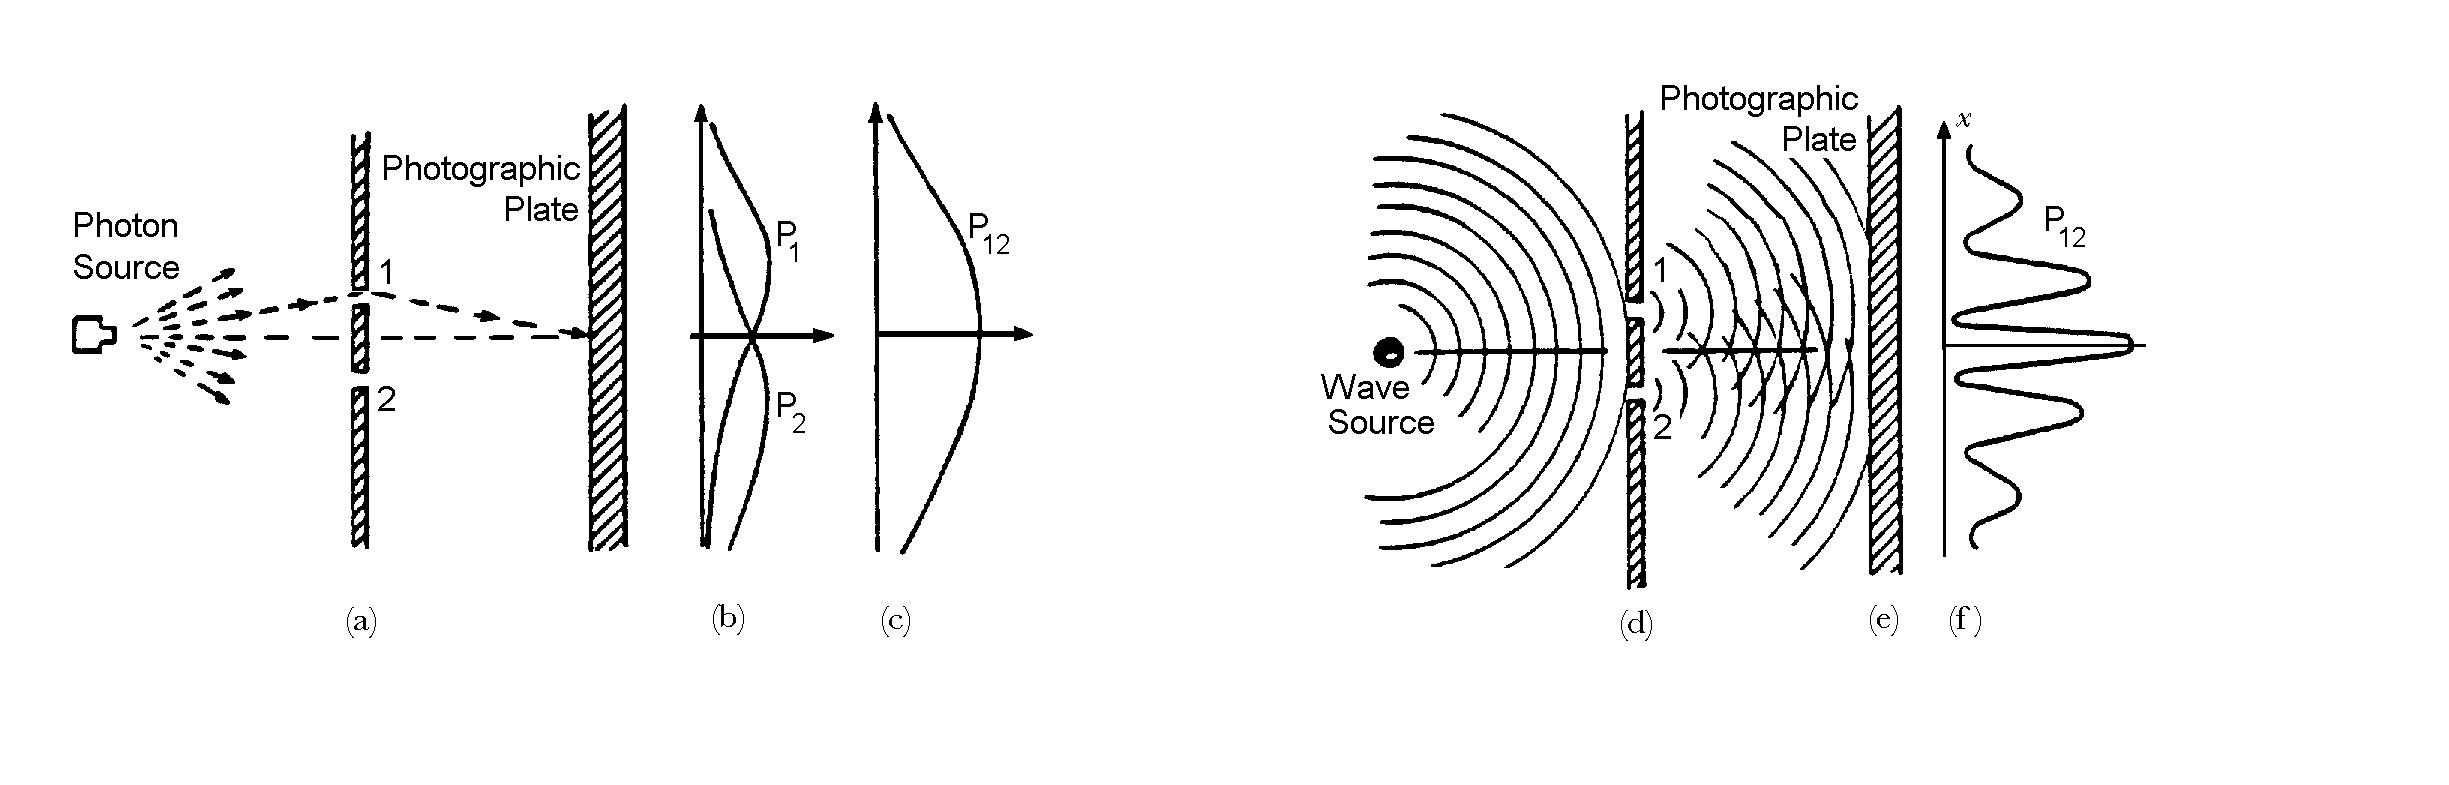
\includegraphics[width=\textwidth,height=.32054\textwidth]{images/10_heisenberg/image058.png}
  \end{center}
  
  } From this we recognize that the assertion that
the photon must have gone either through the one or through the other
hole is problematic and leads to contradictions. This example shows
clearly that the concept of the probability function does not allow a
spatio-temporal description of what happens between two observations.
Any attempt to find such a description would lead to contradictions;
this means that the concept ``happening'' {[}\emph{Geschehen}{]} must be
restricted to observation.

Now, this is surely a very peculiar result, since it seems to indicate
that observation plays a decisive role in the event and that actuality
differs, depending upon whether we observe it or not. To make this point
clearer we have to analyze the process of observation yet more closely.

To begin with, it is important here to recall that in natural science we
are not interested in the universe as a whole, which includes ourselves,
but that we direct our attention to certain parts of the universe and
make those the object of our study. In atomic physics this part is
ordinarily a very small object, namely an atomic particle or a group of
such particles, though sometimes it is much larger; the size does not
here matter. But it \emph{is} important that a large part of the
universe, which includes ourselves, does not belong to the ``object.''

The theoretical interpretation of an experiment starts with\,\ldots two
steps\ldots. In the first step we have to describe the arrangement of
the experiment, if necessary combined with a first observation described
in terms of classical physics, and we have to translate this description
into a probability function. This probability function then satisfies
the laws of quantum theory, and its change in the course of time, which
takes place continuously, can be calculated from the initial conditions.
In this consists the second step. The probability function combines
objective and subjective elements. It contains assertions about
probabilities, or better, tendencies (\emph{potentia} in Aristotelian
philosophy), and these assertions are completely objective; they do not
depend on any observer. It contains, besides, assertions about our
knowledge of the system, which of course have to be subjective insofar
as they can indeed be different for different observers. In especially
favorable cases the subjective element in the probability function can
be quite neglected in comparison with the objective one. The physicists
then speak of a ``pure case.'' {[}\emph{reiner Fall}{]}.

When we now come to the next observation, the result of which was to be
predicted from the theory, it is very important to be clear about the
fact that the object has to interact {[}\emph{in Wechselwirkung
stehen}{]} with the other part of the world, namely, the experimental
device, the measuring rod, etc., before or at least at the moment of
observation. This means that the equation of motion for the probability
function must now take into account the influence which the interaction
with the measuring device exerts on the system. This influence
introduces a new element of indeterminacy, since the measuring device is
necessarily described in the concepts of classical physics. But such a
description contains all the uncertainties concerning the microscopic
structure of the device which we already know from thermodynamics.
Since, besides, the device must be connected with the rest of the world,
it actually contains the uncertainties of the microscopic structure of
the whole world. These uncertainties may be called objective insofar as
they are simply a consequence of the fact that we describe the
experiment in the terms of classical physics; their details do not
depend upon the observer. They may be called subjective insofar as they
indicate our incomplete knowledge of the world.

After this interaction has taken place, the probability function
contains the objective element of a ``tendency'' or ``possibility'' and
the subjective element of incomplete knowledge, even if it had at first
been a matter of a ``pure case.'' It is just for this reason that the
result of the observation cannot generally be predicted with certainty.
What can be predicted is the probability of a certain result of the
observation, and this assertion about the probability can be checked by
repeating the experiment many times. The probability function, unlike
the mathematical formalism of Newtonian mechanics, does not describe a
determinate event but, at least with respect to the process of
observation, a totality of possible events.

The observation itself changes the probability function discontinuously.
It selects from all possible events the one that has actually taken
place. Since through the observation our knowledge of the system has
changed discontinuously, its mathematical representation has also
changed discontinuously, and we therefore speak of a ``quantum leap.''
If someone wanted to derive a criticism of quantum theory from the
ancient saying ``Natura non facit saltus'' {[}nature makes no leaps{]}
we can reply that our \emph{knowledge} can surely change suddenly and
that just this fact, the discontinuous change in our knowledge,
justifies the use of the term ``quantum leap.''

Therefore, the transition from the possible to the actual takes place
during the act of observation. If we want to describe what happens in an
atomic event, we have to begin with the fact that the word ``happens''
can apply only to the observation, not to the situation between two
observations. In doing so, it designates the physical, not the psychical
act of observation, and we may say that the transition from the possible
to the actual takes place as soon as the interaction of the object with
the measuring device, and thereby with the rest of the world, has come
into play. The transition is not connected with the registering of the
observational result in the mind of the observer. The discontinuous
change in the probability function does, to be sure, take place through
the act of registering; for it is that discontinuous change of our
knowledge at the moment of registering which is imaged in the
discontinuous change of the probability function.

\section*{Note\\
  {\large Single-slit Diffraction and the Limit of Optical Resolution}}

1. \emph{Single-slit diffraction}. Let there be a narrow slit of width
$d$, illuminated uniformly along the axis perpendicular to the
plane of the slit. As in Huygens' treatment, consider the plane of the
slit to be populated by infinitely many centers of wavelets, expanding
in all forward directions. Thus the light beam will spread out as it
leaves the slit.

There will be some angle, say $\theta$, at which the wavelets that were
emitted from \emph{one edge} of the slit and from the \emph{center} of
the slit, respectively, will cover distances that differ by an integral
number of half-wavelengths and arrive together at some distant
point---where they will mutually cancel, being exactly out of phase with
one another. The innumerable remaining wavelets may be similarly paired
for mutual cancellation; so that the overall result will be a dark spot
at angle $\theta$ from the perpendicular axis.

In the right triangle thus formed with hypotenuse $d/2$ and one leg
an integral multiple of $\lambda/2$, the marked angle will be equal to
$\theta$ and will have sine given by

\begin{equation*}
\sin \theta = \frac{n\lambda/2}{d/2} = \frac{n\lambda}{d}.
\end{equation*}

Since $n$ is any integer, there will be alternating bands of
illumination and darkness for all angles up to 90$^\circ$ on either side of the
perpendicular axis. But in practice the greatest illumination is found
within the ``central maximum,'' that region bounded by the two minima
for which $n = 1$ (called ``first-order'' minima). Suppose these
minima appear at angles $\theta_1$ on either side of the axis. Then
$\theta_1$ will be the \emph{angular half-width} of the central maximum,
and will be given by

\begin{equation*}
\sin \theta_1 = \frac{\lambda}{d}.
\end{equation*}

2. \emph{Optical resolution}.\footnote{After Curtis Wilson, c. 1980.}
Consider points P$_1$ and P$_2$ on the surface of some object. Let their
angular separation be $\beta$, and let it be supposed that both points
emit or reflect light of wavelength $\lambda$. For the sake of
simplicity, we will let the aperture through which light is admitted to
the instrument be a slit of width $a$ (a circular aperture can be
analogously treated, but numerous complications arise for that case).
Light from each point forms its own independent diffraction pattern with
a central maximum flanked by pairs of minima. As shown in the previous
section 1, each central maximum will have an angular half-width equal to
$\theta_1$ such that

\begin{equation*}
\sin \theta_1 = \lambda/a.
\end{equation*}

Now the central maxima of the two patterns lie in the focal plane of the
instrument lens and (since rays passing through the center of a lens are
not bent) must be separated from one another by the angle $\beta$. But
as aperture \emph{a} is made smaller, the angular half-width of each
central maximum increases, until eventually $\theta_1 = \beta$---that
is, the central maximum of each pattern coincides with a first-order
minimum of the other pattern. The central bright maxima will then be
immediately adjacent to one another. Inspection of the sum of the two
intensity graphs under these conditions shows that instead of forming
two distinct bands, the central maxima will merge into a \emph{single
band}.

Someone viewing such an image through the instrument would be quite
unable to distinguish either of these maxima from the other; and thus
the points P1 and P2 would become \emph{indistinguishable}. No increase
of magnifying power, so long as the same aperture width is retained, can
remedy this limitation. However, if the aperture width $a$ is
increased even the slightest amount, so that the separation between the
two patterns increases by any degree at all, there will be found a dip
between the two maxima when the sum of the intensity graphs is plotted
as before. Thus, that the central maximum of each pattern shall coincide
with the first-order minimum of the other is a \emph{limiting condition}
for the resolution of the images of two points; it is called
\emph{Rayleigh's criterion}.

Heisenberg's equation (16) derives directly from
Rayleigh's criterion. For suppose $\theta_1 = \beta$ as described
above; that is, let
%
\begin{equation}
\sin \beta = \lambda/a. % eqn (1)
\end{equation}
%
Let the object distance be $R$, and suppose also that angle
$\beta$ is very small. Then $\Delta x$ is the chord of a circle with
center at the vertex of $\beta$, and so it very nearly equals the arc
which it subtends. This small arc equals $R\beta$ \ (radians);
while in its turn a very small angle $\beta$ (in radians) nearly equals
$\sin \beta$. This gives $\Delta x \approx R \times \sin\beta$, so that
%
\begin{equation}
\sin \beta \approx \Delta x/R . % eqn (2)
\end{equation}
%
From equations (1) and (2) it follows that
%
\begin{equation}
\frac{\Delta x}{R} = \frac{\lambda}{a}. % eqn (3)
\end{equation}
%


Similarly, the aperture of width $a$ located at distance $R$
from a point will subtend an angle $\varepsilon$ such that, if $\varepsilon$ is
very small,
%
\begin{equation*}
\sin \varepsilon \approx a/R,
\end{equation*}
%
from which

\begin{equation}
a \approx R \sin \varepsilon. % eqn (4)
\end{equation}

Substitution of equation (4) into equation (3) above yields
%
\begin{equation*}
\frac{\Delta x}{R} \approx \frac{\lambda}{R \sin \varepsilon}
\end{equation*}
%
which becomes Heisenberg's equation (16), when $R$ is canceled from
both sides. Q.E.D.

